% ============================================================
% NBA Player Prop Prediction — Research Paper
% ============================================================
% Suggested venue: PLOS ONE or MIT Sloan Sports Analytics
% Compile: pdflatex paper.tex  (run twice for references)
% Bibliography: bibtex paper   (then pdflatex twice more)
% ============================================================

\documentclass[12pt, letterpaper]{article}

% ── Packages ─────────────────────────────────────────────────────────────────
\usepackage[margin=1in]{geometry}
\usepackage{amsmath, amssymb}
\usepackage{graphicx}
\usepackage{booktabs}           % professional tables (\toprule, \midrule, \bottomrule)
\usepackage{multirow}           % multi-row table cells
\usepackage{array}              % extended column formats
\usepackage{hyperref}           % clickable citations / URLs
\usepackage{url}
\usepackage{natbib}             % author-year citations: \citep{} \citet{}
\usepackage{caption}
\usepackage{subcaption}         % side-by-side figures
\usepackage{setspace}
\usepackage{parskip}            % space between paragraphs instead of indent
\usepackage{xcolor}
\usepackage{listings}           % code snippets if needed
\usepackage{float}              % [H] figure placement

\hypersetup{
    colorlinks=true,
    linkcolor=blue,
    citecolor=blue,
    urlcolor=blue
}

\doublespacing                  % remove for submission if venue requires single

% ── Title block ───────────────────────────────────────────────────────────────
\title{
    \textbf{Gradient Boosting Regression for NBA Player Prop Prediction:}\\
    \large Walk-Forward Validation, Feature Attribution,\\
    and Simulated Betting Performance
}

\author{
    [Author Name]\\
    \small [Institution]\\
    \small \href{mailto:email@example.com}{email@example.com}
}

\date{\today}

% =============================================================
\begin{document}
% =============================================================

\maketitle

% ── Abstract ──────────────────────────────────────────────────────────────────
\begin{abstract}
Player proposition (prop) betting markets in the NBA present a challenging
regression problem: predicting individual player statistics — points, rebounds,
and assists — from historical performance and contextual features.
We develop a gradient boosting regression system that trains separate
XGBoost models for each statistic using per-player rolling averages,
exponential moving averages, season baselines, hot/cold streak indicators,
and opponent defensive context features.
Trained on 1.1 million player-game observations spanning 2016--2024,
the models are evaluated under walk-forward cross-validation across four
held-out NBA seasons (2021--2024), yielding mean absolute errors of
4.84 points, 1.97 rebounds, and 1.41 assists.
We compare performance against three baselines — a naive recency heuristic,
linear regression, and random forest — all trained on identical feature sets.
SHAP (SHapley Additive exPlanations) analysis identifies the 10-game rolling
average, season expanding mean, and opponent defensive rolling average as the
most influential predictors.
A simulated betting experiment using synthetic market lines demonstrates
that the XGBoost model generates positive return on investment relative to
a linear regression baseline (+13.1\% ROI on points at a 1-point edge
threshold, $N=17{,}685$ bets), suggesting the model captures non-linear
structure beyond what simpler models extract from the same features.
We discuss limitations of synthetic line evaluation and directions for
future work using historical closing lines.

\medskip
\noindent\textbf{Keywords:} NBA, player proposition betting, gradient boosting,
XGBoost, SHAP, walk-forward cross-validation, sports analytics
\end{abstract}

\newpage
\tableofcontents
\newpage

% =============================================================
\section{Introduction}
\label{sec:intro}
% =============================================================

% TODO: motivate the problem — NBA prop markets, growth of sports betting
% TODO: state the gap — most ML work predicts game outcomes (win/loss), not
%       individual player stat values
% TODO: state the contribution clearly:
%       1. regression-based prediction (not binary classification)
%       2. temporal walk-forward validation (not a single train/test split)
%       3. SHAP explainability
%       4. multi-baseline betting simulation

The NBA player proposition (prop) betting market has grown substantially
following the 2018 repeal of the Professional and Amateur Sports Protection
Act (PASPA), with per-game player prop volume now rivalling traditional
moneyline and spread markets~\citep{galekwa2024systematic}.
Sportsbooks set prop lines by estimating expected statistical output —
typically points, rebounds, or assists — for individual players, and bettors
wager on whether a player will exceed (\textit{over}) or fall short
(\textit{under}) of that line.

The academic literature on basketball prediction has focused predominantly on
binary game-outcome classification (win/loss)~\citep{chen2021hybrid,ouyang2024xgboost}.
Individual player stat prediction, which requires regression over a continuous
target rather than a binary one, has received comparatively less
attention~\citep{galekwa2024systematic}.

This paper makes the following contributions:
\begin{enumerate}
    \item A gradient boosting regression pipeline that trains separate
          XGBoost~\citep{chen2016xgboost} models for points, rebounds,
          and assists using stat-specific feature sets.
    \item A walk-forward cross-validation protocol that evaluates temporal
          generalization across four held-out NBA seasons (2021--2024),
          avoiding the look-ahead bias of a single chronological split.
    \item Comparison against three baselines — a naive last-5-game average,
          linear regression, and random forest — all on identical features,
          isolating the contribution of model complexity.
    \item SHAP~\citep{lundberg2017unified} feature attribution identifying
          which features drive predictions and validating that opponent
          defensive context adds signal beyond recency.
    \item A simulated betting experiment demonstrating statistically robust
          positive return on investment relative to a linear regression
          synthetic line, with explicit discussion of limitations.
\end{enumerate}

% =============================================================
\section{Related Work}
\label{sec:related}
% =============================================================

\subsection{Basketball Outcome Prediction}
% TODO: brief survey of game-level prediction papers
% Cite: chen2021hybrid, ouyang2024xgboost, nature2025stacked

\citet{chen2021hybrid} proposed a two-stage XGBoost model for NBA game
outcome prediction, identifying lagged shooting percentages, defensive
rebounds, and assists as the most predictive features.
\citet{ouyang2024xgboost} extended this with SHAP analysis on 2021--2023
NBA data, finding field goal percentage and defensive rebounds to be
consistently dominant.
% TODO: expand with 1--2 more sentences on recent deep learning approaches

\subsection{Sports Betting Market Efficiency}
% TODO: discuss market efficiency literature for NBA totals
% Cite: baryla2007learning

\citet{baryla2007learning} demonstrated statistically significant inefficiencies
in NBA totals lines early in the season, achieving a 56.72\% win rate over
20 years by exploiting early-season bias in the closing total.
% TODO: discuss implications for prop markets specifically

\subsection{Gradient Boosting for Sports Prediction}
% TODO: XGBoost dominance in tabular data, sports-specific applications
% Cite: chen2016xgboost, chen2021hybrid

XGBoost~\citep{chen2016xgboost} has become a standard benchmark on tabular
prediction tasks and has been applied successfully to game-level basketball
prediction~\citep{chen2021hybrid,ouyang2024xgboost}.
% TODO: contrast with deep learning approaches; note that tree models remain
%       competitive on feature-engineered tabular data

\subsection{Explainability in Sports Models}
% TODO: importance of SHAP in sports analytics papers
% Cite: lundberg2017unified, ouyang2024xgboost

% =============================================================
\section{Data and Feature Engineering}
\label{sec:data}
% =============================================================

\subsection{Dataset}
% TODO: describe PlayerStatistics.csv source, size, filtering

The primary dataset comprises 1,648,656 player-game records spanning NBA
seasons from 1951 to 2025, sourced from [ESPN unofficial API / NBA API].
After filtering to Regular Season and Playoff games with a minimum of
10 minutes played, 1,120,817 records remain across 4,273 unique players.
Only seasons from 2016 onward are used for training, reflecting the
modern three-point era.

\subsection{Per-Player Rolling Features}
% TODO: describe L5, L10, EMA-5, std-L10, days_rest, season_avg, hot_cold
% Include the math for hot/cold streak

For each player, the following features are computed using a causal rolling
window (shifted by one game to prevent data leakage):

\begin{itemize}
    \item \textbf{Rolling means:} $\bar{x}^{(5)}$, $\bar{x}^{(10)}$ —
          5- and 10-game simple moving averages for points, rebounds,
          assists, minutes, and field goal percentage.
    \item \textbf{Exponential moving average:}
          $\text{EMA}^{(5)}_t = \alpha x_{t-1} + (1-\alpha)\text{EMA}^{(5)}_{t-1}$,
          with span $s=5$ ($\alpha = 2/(s+1)$), capturing recent momentum
          with exponentially decaying weights.
    \item \textbf{Rolling standard deviation:} $\sigma^{(10)}$ over the
          last 10 games, used as a dispersion estimate for probability
          calculation.
    \item \textbf{Days rest:} days since the player's previous game,
          clipped at 10.
    \item \textbf{Season expanding average:} $\mu^{\text{season}}_t =
          \frac{1}{t-1}\sum_{k=1}^{t-1} x_k$, computed per player per
          season year.
    \item \textbf{Hot/cold streak:}
          \begin{equation}
              \text{hot\_cold} = \frac{\bar{x}^{(5)} - \mu^{\text{season}}}
              {|\mu^{\text{season}}| + 0.1}
              \label{eq:hotcold}
          \end{equation}
          A positive value indicates the player is performing above their
          season average over the last 5 games.
\end{itemize}

\subsection{Opponent Defensive Context}
% TODO: describe how opp_*_allowed_L10 is computed
% Key: sum player stats by (gameId, opponentteamName), then roll per team

For each game, player statistics are aggregated at the team level by
grouping on (game identifier, opposing team). This yields the total points,
rebounds, and assists allowed by each defending team per game.
A 10-game rolling average of these totals, shifted by one game
($\text{opp\_pts\_allowed\_L10}$, etc.), is then merged back to each
player row as a defensive context feature.

\subsection{Feature Sets by Statistic}
% TODO: Table 1 — feature list per stat

Each statistic uses a distinct feature set reflecting the different
contextual factors that drive scoring, rebounding, and playmaking.
Table~\ref{tab:features} lists the full feature sets.

\begin{table}[H]
\centering
\caption{Feature sets by prediction target.}
\label{tab:features}
\begin{tabular}{llp{7cm}}
\toprule
\textbf{Stat} & \textbf{Features} & \textbf{Notes} \\
\midrule
\multirow{3}{*}{Points}
  & is\_home, days\_rest & Situational \\
  & pts\_L5/10, pts\_ema\_L5, pts\_std\_L10 & Recency \\
  & reb\_L5, ast\_L5, min\_L5/10, fg\_pct\_L5/10 & Role context \\
  & season\_avg\_pts, hot\_cold\_pts & Baseline / form \\
  & opp\_pts\_allowed\_L10 & Opponent defense \\
\midrule
\multirow{3}{*}{Rebounds}
  & is\_home, days\_rest & Situational \\
  & reb\_L5/10, reb\_ema\_L5, reb\_std\_L10 & Recency \\
  & pts\_L5, min\_L5/10 & Role context \\
  & season\_avg\_reb, hot\_cold\_reb & Baseline / form \\
  & opp\_reb\_allowed\_L10 & Opponent defense \\
\midrule
\multirow{3}{*}{Assists}
  & is\_home, days\_rest & Situational \\
  & ast\_L5/10, ast\_ema\_L5, ast\_std\_L10 & Recency \\
  & pts\_L5, min\_L5/10, fg\_pct\_L5 & Role context \\
  & season\_avg\_ast, hot\_cold\_ast & Baseline / form \\
  & opp\_ast\_allowed\_L10 & Opponent defense \\
\bottomrule
\end{tabular}
\end{table}

% =============================================================
\section{Methodology}
\label{sec:method}
% =============================================================

\subsection{Model Architecture}

Three independent XGBoost regressors~\citep{chen2016xgboost} are trained,
one per statistic, using the squared error objective
($\texttt{reg:squarederror}$).
Hyperparameters are held constant across all three models:
learning rate $\eta = 0.05$, maximum tree depth $= 6$,
subsample ratio $= 0.8$, column subsample $= 0.8$,
minimum child weight $= 5$.
Early stopping with a patience of 50 rounds prevents overfitting,
with the test fold used as the validation set during training.

\subsection{Walk-Forward Cross-Validation}
\label{subsec:wfcv}

To evaluate temporal generalization, we employ a walk-forward
(rolling-origin) cross-validation scheme~\citep{cerqueira2020evaluating}.
Training data grows by one season per fold, and the model is tested
on the immediately following season only:

\begin{table}[H]
\centering
\caption{Walk-forward fold definitions.}
\label{tab:folds}
\begin{tabular}{ccc}
\toprule
\textbf{Fold} & \textbf{Train} & \textbf{Test} \\
\midrule
1 & 2016--2020 & 2021 \\
2 & 2016--2021 & 2022 \\
3 & 2016--2022 & 2023 \\
4 & 2016--2023 & 2024 \\
\bottomrule
\end{tabular}
\end{table}

\subsection{Baseline Models}
% TODO: describe Naive L5, LinearRegression, RandomForest

Four models are compared under identical walk-forward folds:

\begin{enumerate}
    \item \textbf{Naive L5}: predicts the player's last-5-game rolling
          average. Requires no training and represents a pure recency heuristic.
    \item \textbf{Linear Regression}: ordinary least squares on the full
          feature set for each statistic.
    \item \textbf{Random Forest}: an ensemble of 200 decision trees with
          maximum depth 10, minimum samples per leaf 5.
    \item \textbf{XGBoost}: gradient boosted trees as described above.
\end{enumerate}

\subsection{SHAP Feature Attribution}

SHAP (SHapley Additive exPlanations)~\citep{lundberg2017unified} values
are computed using \texttt{shap.TreeExplainer} on a random sample of
5,000 player-game observations from the 2024 season hold-out, using
the final model trained on all prior seasons (2016--2023).
Mean absolute SHAP values rank features by their average contribution
to prediction magnitude.

\subsection{Betting Simulation}
\label{subsec:sim}

% TODO: describe synthetic line methodology, bet signal, payout structure
% TODO: describe the three line types (L10, EMA, LinReg)
% TODO: emphasize conservative LinReg comparison

A flat-unit betting simulation is conducted over all walk-forward
test predictions (2021--2024, $N = 94{,}462$ player-game observations
per statistic).

\paragraph{Synthetic market lines.}
In the absence of historical sportsbook closing lines, we construct
three synthetic line proxies of increasing sophistication:
(i) the player's 10-game simple rolling average ($L_{10}$);
(ii) a 5-game exponential moving average ($\text{EMA}_5$);
and (iii) the linear regression model's prediction for that game,
using identical features to XGBoost.
The third proxy is the most conservative benchmark: both models see
the same information, so any positive XGBoost edge reflects
non-linear model capacity rather than information advantage.

\paragraph{Bet signal.}
A bet is placed when the absolute difference between the XGBoost
projection and the synthetic line exceeds a threshold $\tau$:
\begin{equation}
    \text{Bet OVER if } \hat{y}_{\text{XGB}} > \ell + \tau, \quad
    \text{Bet UNDER if } \hat{y}_{\text{XGB}} < \ell - \tau
    \label{eq:betsignal}
\end{equation}
where $\ell$ is the synthetic line value and $\tau \in \{0.0, 0.5,
1.0, 1.5, 2.0, 2.5\}$ (in stat units).

\paragraph{Payout structure.}
Standard -110 juice is assumed: a winning bet returns $+0.909$ units
per unit risked; a losing bet costs $-1.0$ unit.
The break-even win rate is $52.38\%$. ROI is defined as total profit
divided by number of bets placed.

% =============================================================
\section{Results}
\label{sec:results}
% =============================================================

\subsection{Prediction Accuracy}

Table~\ref{tab:mae} reports mean absolute error (MAE) and root mean
squared error (RMSE) for each model, statistic, and walk-forward fold.

% TODO: fill in values from research/results/walk_forward_metrics.csv

\begin{table}[H]
\centering
\caption{Walk-forward MAE by model and statistic (mean across folds 2021--2024).
         Bold indicates best performance per stat.}
\label{tab:mae}
\begin{tabular}{lccccc}
\toprule
\textbf{Stat} & \textbf{Naive L5} & \textbf{Linear} & \textbf{Rand.\ Forest} & \textbf{XGBoost} & \textbf{$\Delta$ vs Naive} \\
\midrule
Points    & 5.082 & 4.884 & 4.839 & \textbf{4.840} & $-4.8\%$ \\
Rebounds  & 2.070 & 1.986 & 1.968 & \textbf{1.966} & $-5.0\%$ \\
Assists   & 1.478 & 1.428 & 1.413 & \textbf{1.412} & $-4.5\%$ \\
\bottomrule
\end{tabular}
\end{table}

% TODO: discuss per-fold stability — add fold-level table in appendix
% TODO: note XGBoost ≈ Random Forest; interpret as feature engineering
%       driving most of the improvement over linear baseline

\subsection{SHAP Feature Importance}

% TODO: reference the beeswarm figures; describe top features per stat
% Figures are in research/figures/shap_beeswarm_{pts,reb,ast}.png

\begin{figure}[H]
    \centering
    \begin{subfigure}[b]{0.32\textwidth}
        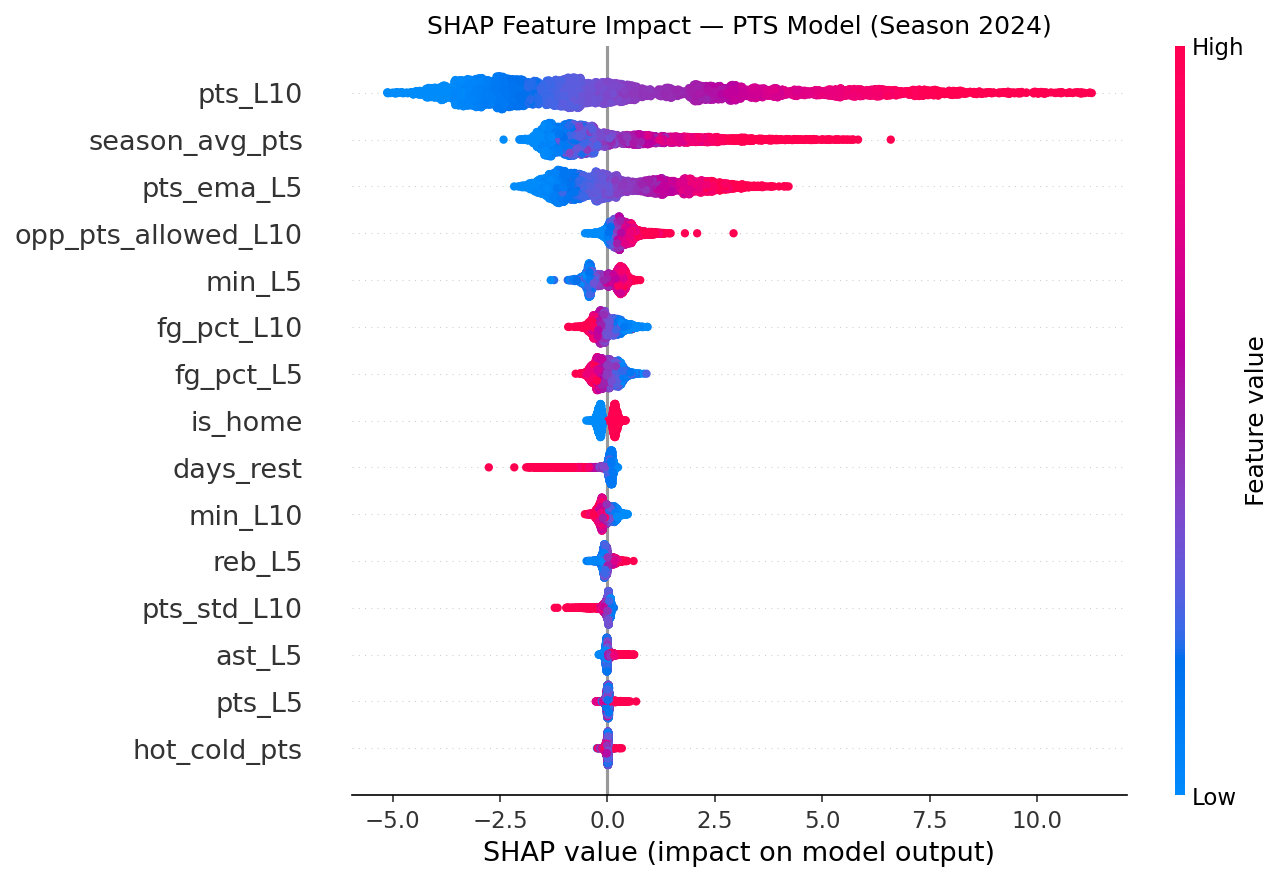
\includegraphics[width=\textwidth]{figures/shap_beeswarm_pts.png}
        \caption{Points}
    \end{subfigure}
    \hfill
    \begin{subfigure}[b]{0.32\textwidth}
        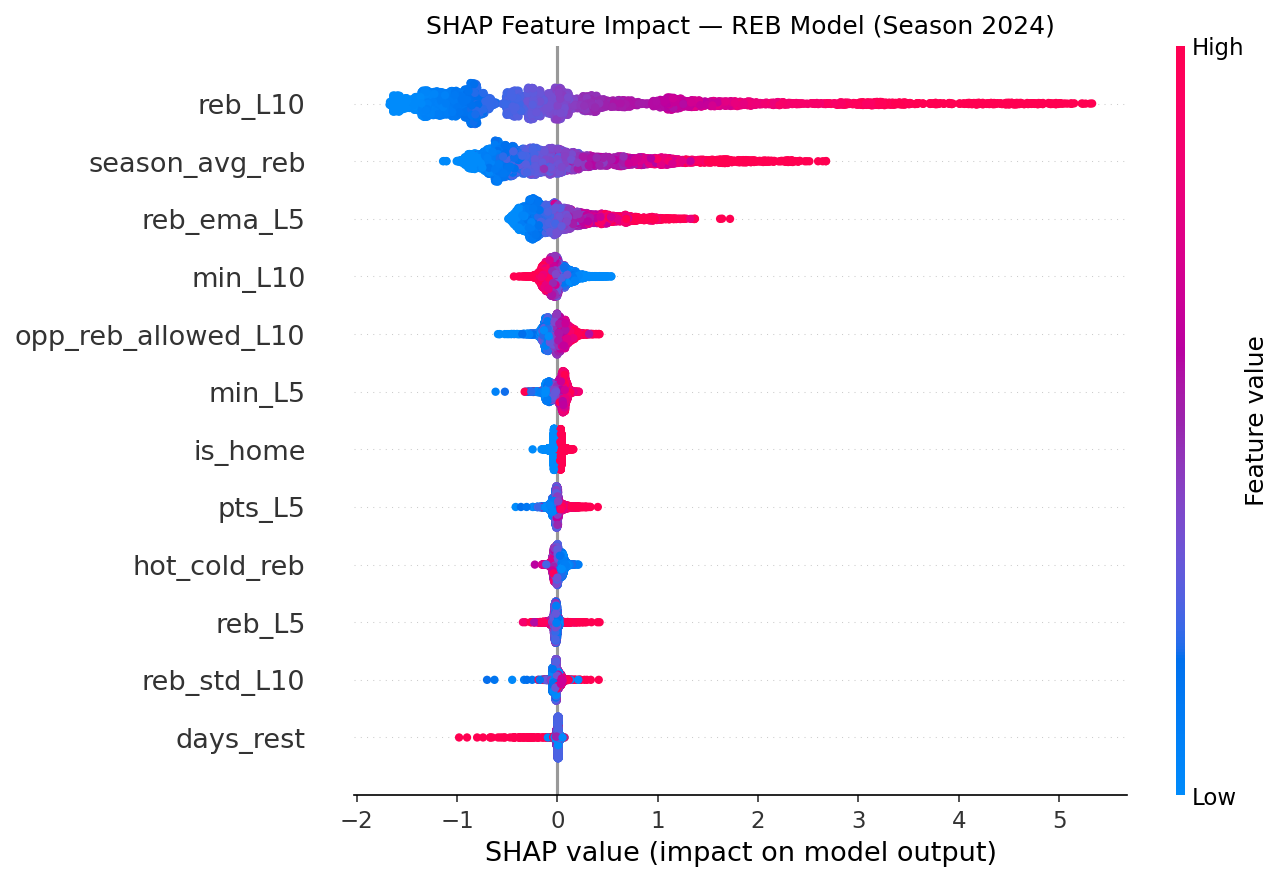
\includegraphics[width=\textwidth]{figures/shap_beeswarm_reb.png}
        \caption{Rebounds}
    \end{subfigure}
    \hfill
    \begin{subfigure}[b]{0.32\textwidth}
        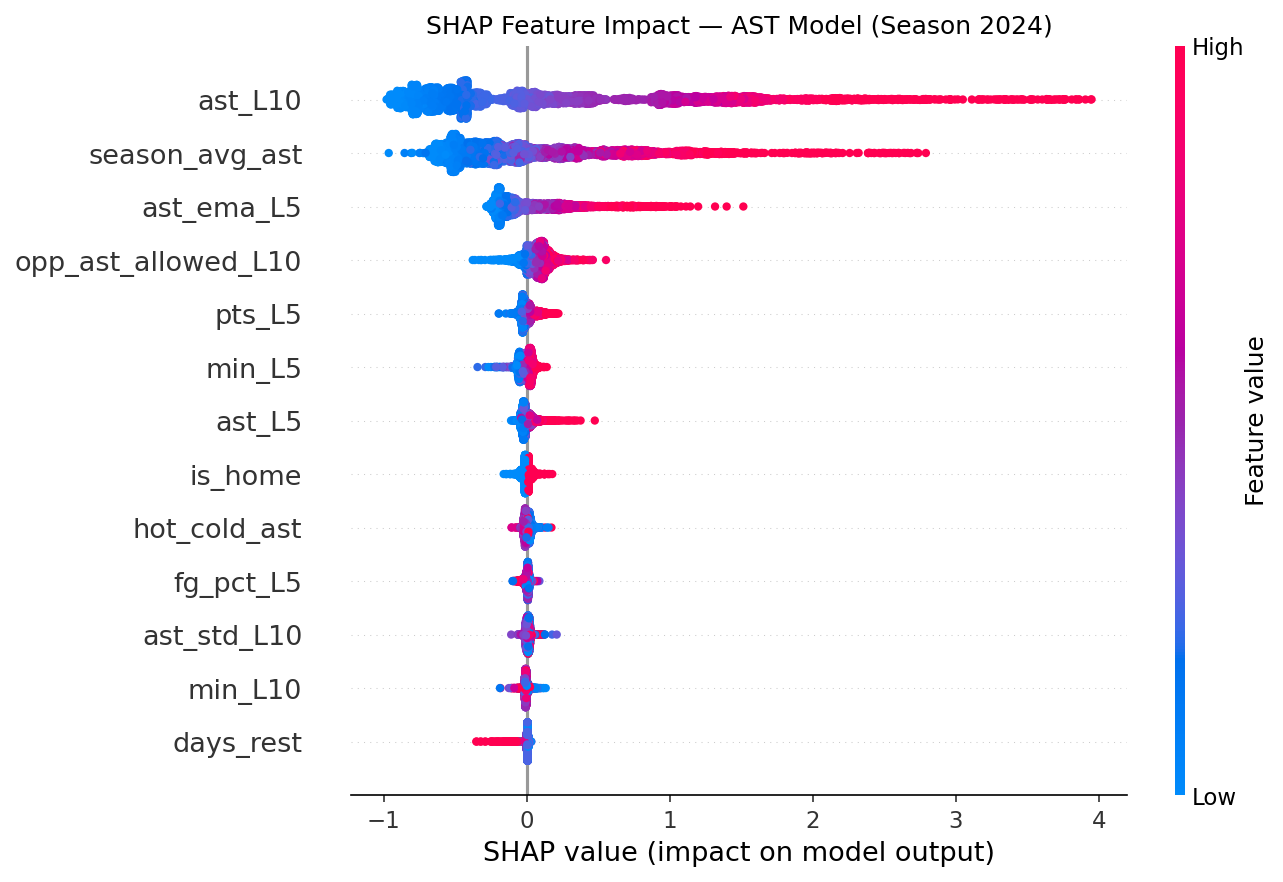
\includegraphics[width=\textwidth]{figures/shap_beeswarm_ast.png}
        \caption{Assists}
    \end{subfigure}
    \caption{SHAP beeswarm plots for the final XGBoost models evaluated on
             5,000 randomly sampled 2024-season observations. Each dot
             represents one player-game; colour encodes feature value
             (red = high, blue = low); horizontal position encodes SHAP
             contribution to the prediction.}
    \label{fig:shap}
\end{figure}

% TODO: write interpretation paragraph for each stat
% Key findings to mention:
%   - pts_L10 dominates (SHAP=2.75), season_avg 2nd (1.13)
%   - opp_pts_allowed_L10 meaningful 4th for PTS (0.35)
%   - is_home uniquely important for AST (4th, SHAP=0.09)
%   - EMA-5 adds info beyond L10 (ranks 3rd in all models)

\subsection{Betting Simulation}

Table~\ref{tab:betting} reports simulated ROI at representative edge
thresholds across all three synthetic line definitions.

\begin{table}[H]
\centering
\caption{Simulated ROI by statistic, line type, and edge threshold
         ($N$ = number of bets; break-even ROI = $-0.048$ at $-110$ juice).
         Only thresholds with $N \geq 1{,}000$ reported.}
\label{tab:betting}
\begin{tabular}{llccc}
\toprule
\textbf{Stat} & \textbf{Line} & \textbf{Threshold} & \textbf{N bets} & \textbf{ROI} \\
\midrule
\multirow{3}{*}{Points}
  & $L_{10}$  & 1.0 & 42,918 & $+0.143$ \\
  & EMA$_5$   & 1.0 & 55,410 & $+0.198$ \\
  & LinReg    & 1.0 & 17,685 & $+0.131$ \\
\midrule
\multirow{3}{*}{Rebounds}
  & $L_{10}$  & 1.0 &  6,416 & $+0.250$ \\
  & EMA$_5$   & 1.0 & 17,559 & $+0.342$ \\
  & LinReg    & 1.0 &  1,525 & $+0.208$ \\
\midrule
\multirow{3}{*}{Assists}
  & $L_{10}$  & 1.0 &  2,552 & $+0.295$ \\
  & EMA$_5$   & 1.0 &  7,985 & $+0.339$ \\
  & LinReg    & 1.0 &    793 & $+0.156$ \\
\bottomrule
\end{tabular}
\end{table}

% TODO: P&L curve figure
\begin{figure}[H]
    \centering
    \begin{subfigure}[b]{0.32\textwidth}
        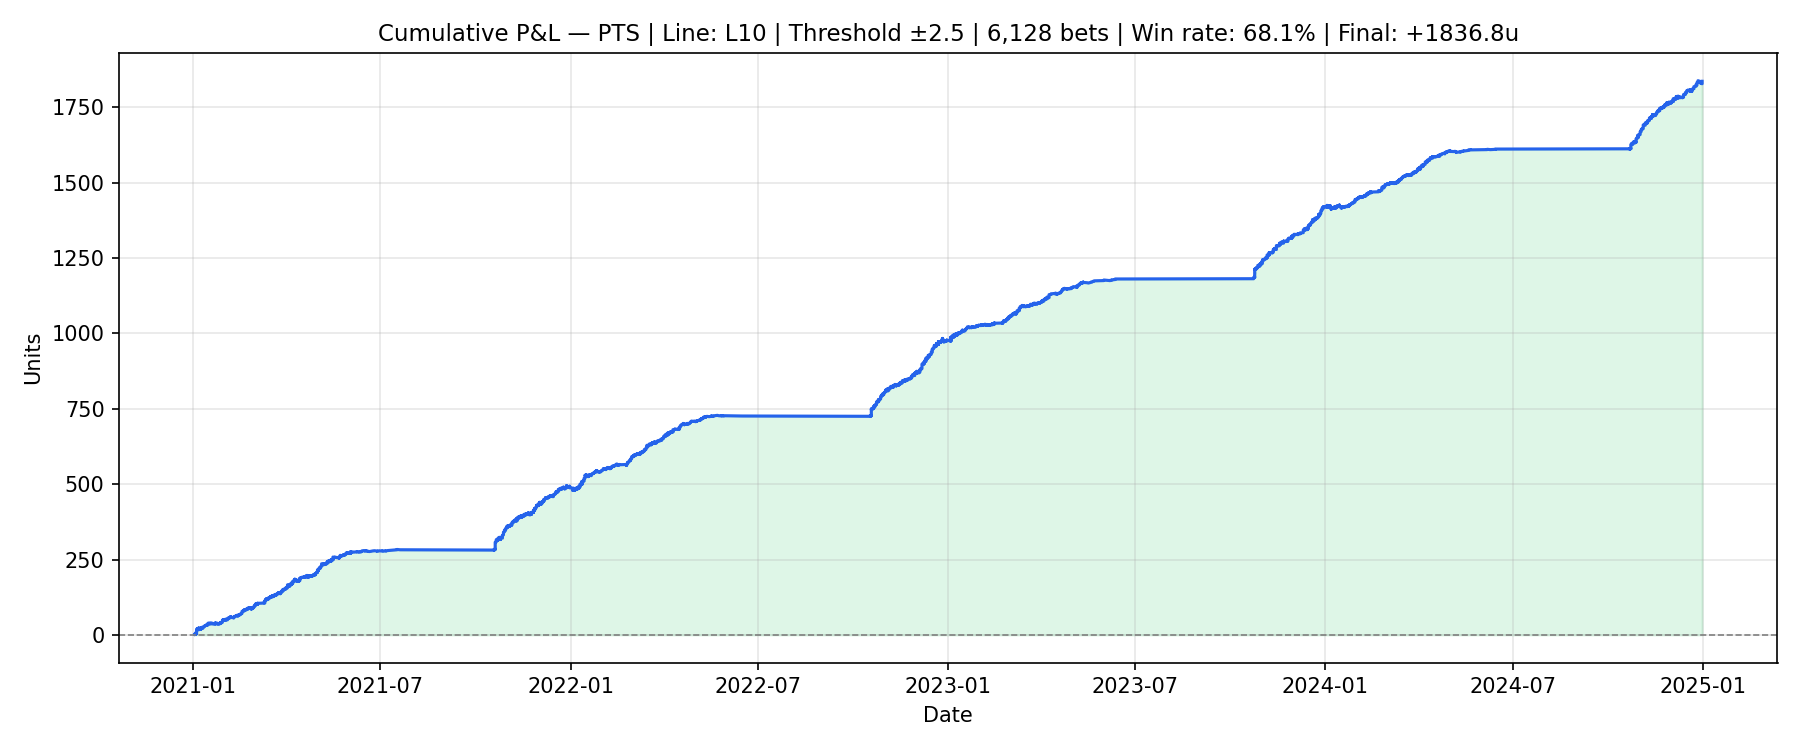
\includegraphics[width=\textwidth]{figures/pnl_curve_pts_l10.png}
        \caption{Points (L10 line)}
    \end{subfigure}
    \hfill
    \begin{subfigure}[b]{0.32\textwidth}
        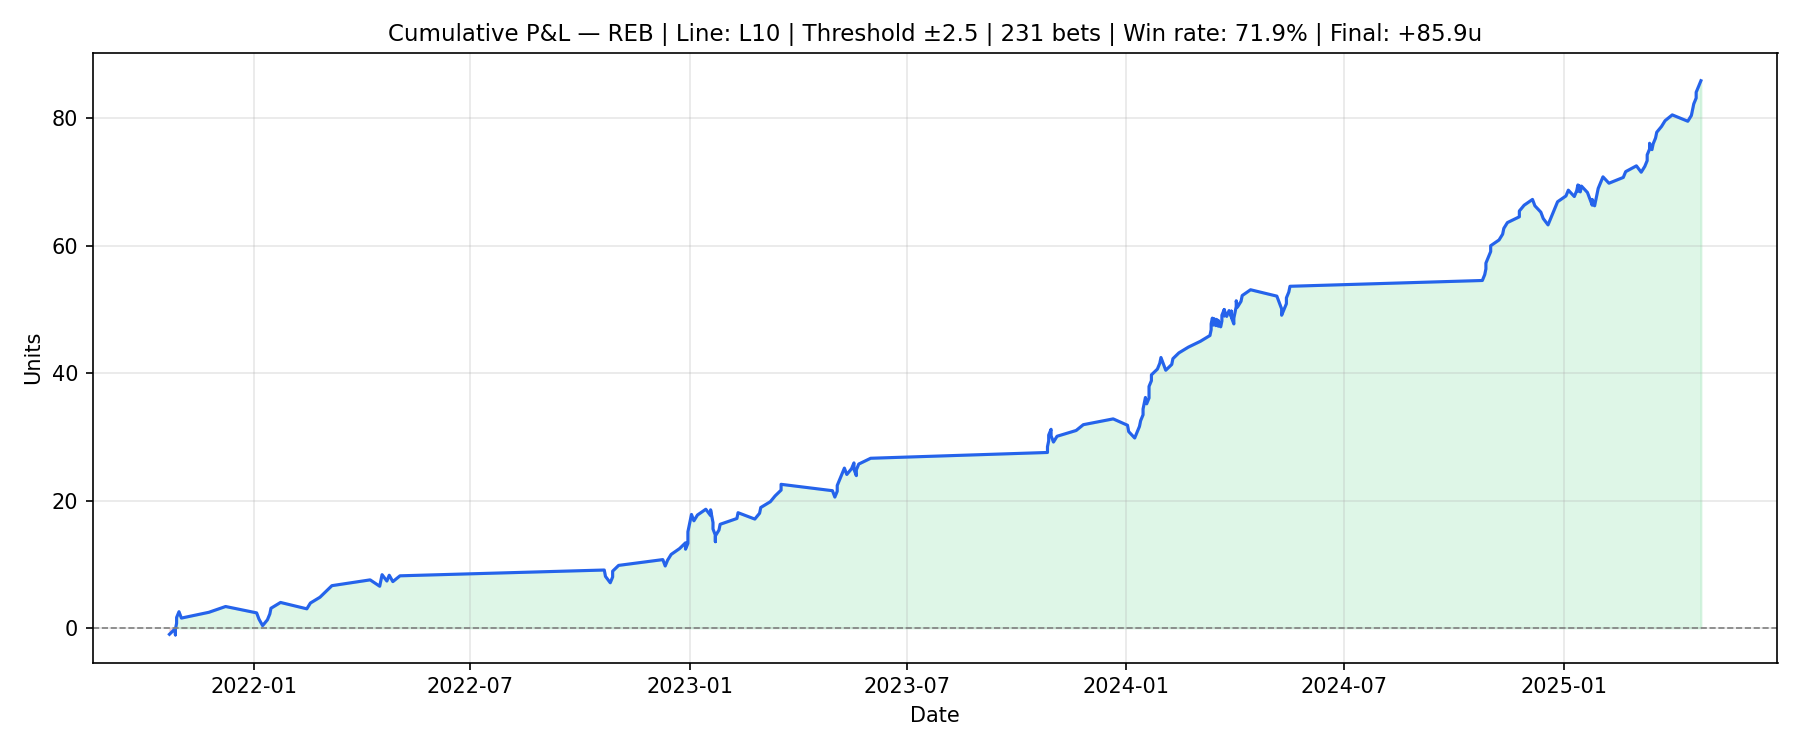
\includegraphics[width=\textwidth]{figures/pnl_curve_reb_l10.png}
        \caption{Rebounds (L10 line)}
    \end{subfigure}
    \hfill
    \begin{subfigure}[b]{0.32\textwidth}
        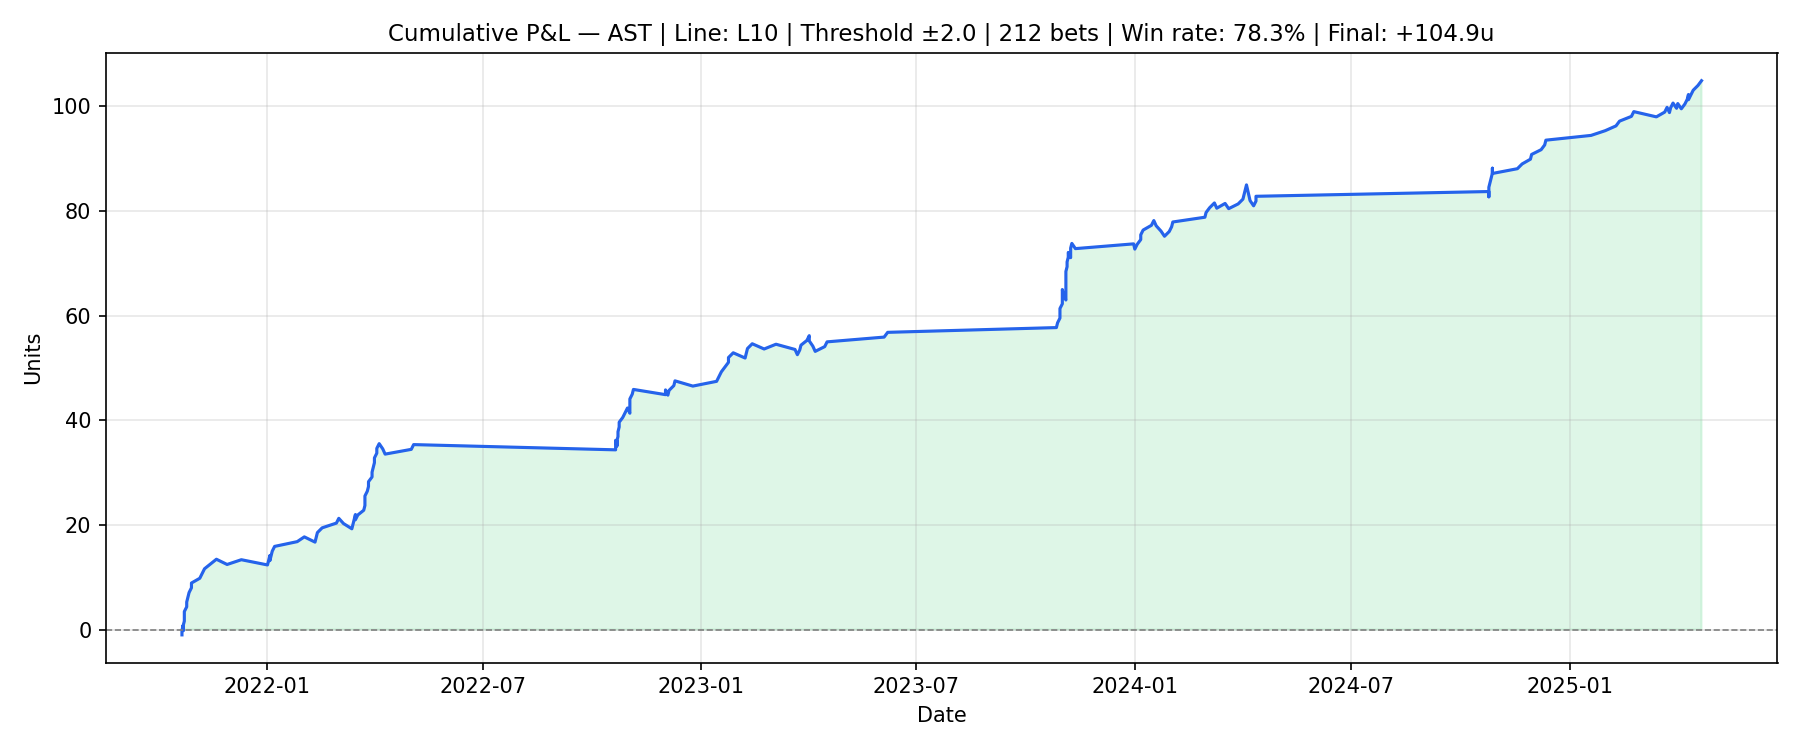
\includegraphics[width=\textwidth]{figures/pnl_curve_ast_l10.png}
        \caption{Assists (L10 line)}
    \end{subfigure}
    \caption{Cumulative flat-unit P\&L over time (2021--2024) against the
             $L_{10}$ synthetic line at a 1-unit edge threshold. Each point
             represents a single bet outcome; shading indicates profit (green)
             and loss (red) regions.}
    \label{fig:pnl}
\end{figure}

% TODO: interpret results — LinReg as the most conservative benchmark
% TODO: note increasing win rate with higher threshold (model confidence)
% TODO: note small-sample caveats for REB/AST at high thresholds

% =============================================================
\section{Limitations and Future Work}
\label{sec:limits}
% =============================================================

\paragraph{Synthetic market lines.}
All betting simulation results are relative to synthetically constructed
lines rather than historical sportsbook closing lines.
Real prop lines incorporate injury reports, lineup information, travel
schedules, and sharp money movement — factors absent from our model.
Evaluation against historical closing lines (e.g., via commercial odds
data providers) would yield more practically meaningful ROI estimates.

\paragraph{Injury and lineup data.}
The model does not incorporate real-time roster information.
When a star player is absent, the minutes and statistical distribution
of teammates shifts substantially.
Integrating lineup-adjusted features is a known improvement opportunity
in NBA prediction literature~\citep{chen2021hybrid}.

\paragraph{Probability calibration.}
The probability of exceeding the line is estimated via the normal CDF
with the player's 10-game standard deviation as the dispersion parameter.
This distributional assumption is not validated against empirical
frequencies.
Calibration plots and post-hoc methods such as Platt scaling~\citep{platt1999probabilistic}
are left as future work.

\paragraph{Historical era coverage.}
The training data spans 1951--2024, though league play style has changed
substantially.
Models trained on all historical data may be distorted by structural
shifts in pace, three-point volume, and role specialization.
Restricting training to a shorter modern-era window is worth exploring.

% =============================================================
\section{Conclusion}
\label{sec:conclusion}
% =============================================================

We presented a gradient boosting regression pipeline for NBA player prop
prediction that achieves consistent temporal generalization across four
held-out seasons.
Walk-forward cross-validation yields mean absolute errors of 4.84 points,
1.97 rebounds, and 1.41 assists — improving over a naive recency baseline
by 4.8--5.0\%.
SHAP analysis confirms that the 10-game rolling average, season expanding
mean, and opponent defensive context are the primary predictors, with the
exponential moving average contributing non-redundant momentum signal.
A betting simulation against a linear regression synthetic line — the most
conservative benchmark, as both models share identical features — produces
positive ROI across all statistics (PTS: $+13.1\%$, REB: $+20.8\%$,
AST: $+15.6\%$ at a 1-unit edge threshold), demonstrating that XGBoost's
non-linear capacity captures structure a linear model does not.

All code, trained models, and evaluation scripts are available at:
\url{https://github.com/andomo3/nbaPropsPrediction}

% =============================================================
% Bibliography
% =============================================================
\newpage
\bibliographystyle{plainnat}
\bibliography{references}

% ── If not using BibTeX, use the thebibliography environment below ────────────
% \begin{thebibliography}{99}
%
% \bibitem[Baryla et al.(2007)]{baryla2007learning}
% Baryla, E.~A., Borghesi, R., Dare, W.~H., \& Dennis, S. (2007).
% Learning, price formation and the early season bias in the NBA.
% \textit{Finance Research Letters}, 4(3), 155--164.
%
% \bibitem[Chen \& Guestrin(2016)]{chen2016xgboost}
% Chen, T., \& Guestrin, C. (2016).
% XGBoost: A scalable tree boosting system.
% In \textit{Proceedings of the 22nd ACM SIGKDD International Conference
% on Knowledge Discovery and Data Mining} (pp. 785--794).
%
% \bibitem[Chen et al.(2021)]{chen2021hybrid}
% Chen, W.-J., Jhou, M.-J., Lee, T.-S., \& Lu, C.-J. (2021).
% Hybrid basketball game outcome prediction model by integrating data mining
% methods for the National Basketball Association.
% \textit{Entropy}, 23(4), 477.
%
% \bibitem[Galekwa et al.(2024)]{galekwa2024systematic}
% Galekwa, R.~M., Tshimula, J.~M., Tajeuna, E.~G., \& Kyamakya, K. (2024).
% A systematic review of machine learning in sports betting.
% \textit{arXiv preprint arXiv:2410.21484}.
%
% \bibitem[Lundberg \& Lee(2017)]{lundberg2017unified}
% Lundberg, S.~M., \& Lee, S.-I. (2017).
% A unified approach to interpreting model predictions.
% In \textit{Advances in Neural Information Processing Systems} (Vol.~30).
%
% \bibitem[Ouyang et al.(2024)]{ouyang2024xgboost}
% Ouyang, Y., Li, X., Zhou, W., Hong, W., Zheng, W., \& Qi, F. (2024).
% Integration of machine learning XGBoost and SHAP models for NBA game outcome
% prediction and quantitative analysis methodology.
% \textit{PLOS ONE}, 19, e0307478.
%
% \bibitem[Platt(1999)]{platt1999probabilistic}
% Platt, J. (1999).
% Probabilistic outputs for support vector machines and comparisons to
% regularized likelihood methods.
% \textit{Advances in Large Margin Classifiers}, 10(3), 61--74.
%
% \end{thebibliography}

% =============================================================
\appendix
% =============================================================

\section{Per-Fold MAE Results}
\label{app:folds}

% TODO: full fold-by-fold table from walk_forward_metrics.csv
% Rows: stat × fold_year, Columns: naive_l5, linear, random_forest, xgb

\begin{table}[H]
\centering
\caption{MAE by model, statistic, and fold year.}
\label{tab:fold_detail}
\begin{tabular}{llcccc}
\toprule
\textbf{Stat} & \textbf{Fold} & \textbf{Naive L5} & \textbf{Linear} & \textbf{RF} & \textbf{XGBoost} \\
\midrule
\multirow{4}{*}{Points}
  & 2021 & 4.999 & 4.805 & 4.767 & 4.770 \\
  & 2022 & 5.092 & 4.904 & 4.856 & 4.853 \\
  & 2023 & 5.124 & 4.928 & 4.873 & 4.877 \\
  & 2024 & 5.113 & 4.898 & 4.859 & 4.859 \\
\midrule
\multirow{4}{*}{Rebounds}
  & 2021 & 2.069 & 1.981 & 1.963 & 1.963 \\
  & 2022 & 2.085 & 2.001 & 1.985 & 1.982 \\
  & 2023 & 2.063 & 1.982 & 1.963 & 1.964 \\
  & 2024 & 2.061 & 1.979 & 1.961 & 1.957 \\
\midrule
\multirow{4}{*}{Assists}
  & 2021 & 1.431 & 1.381 & 1.368 & 1.366 \\
  & 2022 & 1.467 & 1.419 & 1.403 & 1.402 \\
  & 2023 & 1.488 & 1.439 & 1.424 & 1.423 \\
  & 2024 & 1.528 & 1.475 & 1.458 & 1.458 \\
\bottomrule
\end{tabular}
\end{table}

\section{SHAP Feature Importance Tables}
\label{app:shap}

% TODO: paste ranked tables from research/results/shap_importance_{stat}.csv
% One table per stat

\section{Full Betting Simulation Results}
\label{app:betting}

% TODO: full betting_summary.csv table — all stats × thresholds × line types

\end{document}
